\documentclass{beamer}

%\usepackage[utf8]{inputenc} 
%\usepackage[T1]{fontenc}
%\usepackage{lmodern}
%\usepackage{graphicx}
\usepackage[english]{babel}
%\usepackage{array}
%\usepackage{multirow}
%\usepackage{caption}
%\usepackage{fixltx2e}
\usepackage{listings}
%\setbeamertemplate{bibliography item}{[\theenumiv]}
\usepackage[outputdir=figs]{diagrams-latex}

\usetheme[]{Berkeley} %backgroundimagefile=figs/logo.png, useblacktitletext

\begin{document}

\lstset{
  language=Haskell,
  keywordstyle=\color{blue},
  basicstyle=\small\sffamily,
  columns=fullflexible,
  showstringspaces=false,
  mathescape=true,
  captionpos=b
}

\title{Presentation of Haskell}
\subtitle{Hackerspace Trento}
\author{Corentin Dupont}

\date{March 19, 2014}

\maketitle

\begin{frame}
  \frametitle{Table of Contents}
  \begin{columns}[]
   \begin{column}[]{5cm}
    \tableofcontents[]
   \end{column}
   \begin{column}[]{5cm}
    
\includegraphics[width=1\linewidth]{figs/xkcd}
   \end{column}
  \end{columns}
\end{frame}

\section{Motivation}

\begin{frame}[fragile]
\frametitle{What does this code do?}

\begin{lstlisting}[language=C, basicstyle=\tiny]
void f(int a[], int lo, int hi) 
{
  int h, l, p, t;

  if (lo < hi) {
    l = lo;
    h = hi;
    p = a[hi];

    do {
      while ((l < h) && (a[l] <= p)) 
          l = l+1;
      while ((h > l) && (a[h] >= p))
          h = h-1;
      if (l < h) {
          t = a[l];
          a[l] = a[h];
          a[h] = t;
      }
    } while (l < h);

    a[hi] = a[l];
    a[l] = p;

    f( a, lo, l-1 );
    f( a, l+1, hi );
  }
\end{lstlisting}

\end{frame}

\begin{frame}[fragile]
\frametitle{The same in Haskell}

\begin{lstlisting}
  qsort []     = []
  qsort (p:xs) = (qsort lesser) ++ [p] ++ (qsort greater)
    where
        lesser  = filter (< p) xs
        greater = filter (>= p) xs

\end{lstlisting}

\end{frame}

\begin{frame}
\frametitle{Motivation}

 \begin{itemize}
  \item 10 time less lines than in C,
  \item Great expressivity,
  \item Great genericity,
  \item More readable, more maintainable,
  \item Very few bugs: if it compiles, 90\% chances it works on the first try
 \end{itemize}
 
\end{frame}


\section{Features}
\begin{frame}
\frametitle{Features}

 \begin{itemize}
  \item Functional
  \item Pure
  \item Statically typed
  \item Lazy
 \end{itemize}

\end{frame}

\subsection{Functional}
\begin{frame}[fragile]
\frametitle{Functional}

 \begin{itemize}
  \item Functions are first order values
  \item Anonymous functions
  \item Partial application
 \end{itemize}

 \vspace{0.5cm}
 \begin{block}{Examples}
  \begin{lstlisting} 
   myFunc a = a + 1
  
   map (+1) [1..10]
  
   filter (>3) [1, 4, 5, 2]
  
   zip [1, 2, 3] ['a', 'b', 'c']
  
  \end{lstlisting}
 \end{block}

\end{frame}

\begin{frame}[fragile]
\frametitle{Functional}
 
 \begin{itemize}
  \item Lambda functions
  \item Pattern matching	  
 \end{itemize}

 \vspace{0.5cm}
 \begin{block}{Examples}

  \begin{lstlisting} 
   map (\a -> a + 1) [1..10]
  
   fib 0 = 0
   fib 1 = 1
   fib n = fib (n - 2) + fib (n - 1)
  
  \end{lstlisting}
 \end{block}

\end{frame}

\subsection{Pure}
\begin{frame}[fragile]
\frametitle{Pure}

 \begin{columns}[]
  \begin{column}[]{5cm}
   \begin{itemize}
    \item Functions don't read from environment
    \item Functions don't write to environment
   \end{itemize}
  \end{column}
  \begin{column}[]{5cm}
    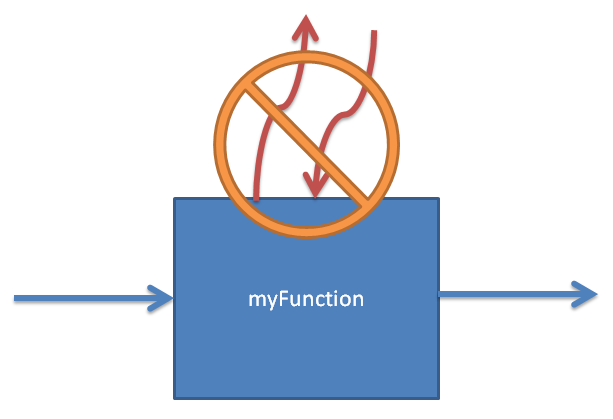
\includegraphics[width=0.8\linewidth]{figs/pure}
  \end{column}
 \end{columns}
 \vspace{0.3cm}
 The output of a function will always be the same for a given input.
 
 \begin{block}{Counter examples in C}
  \begin{lstlisting}[language=C]
    a = f() + g() 
  \end{lstlisting}
  Can we refactor this into a = g() + f()?

  \begin{lstlisting}[language=C]
    a = b 
  \end{lstlisting}
  Can I replace a by b in all my code?

 \end{block}
 
\end{frame}

\begin{frame}
\frametitle{Pure}

 \begin{columns}[]
  \begin{column}[]{5cm}
   \begin{itemize}
    \item No variables!
    \item No for loops!
    \item No assignment operator!
    \item Order of instructions doesn't matter
   \end{itemize}
  \end{column}
  \begin{column}[]{5cm}
    
\includegraphics[width=0.7\linewidth]{figs/neo}
  \end{column}
 \end{columns}
 \vspace{0.5cm}
 
\end{frame}

\begin{frame}
\frametitle{Pure}

What do I win with purity?
 \begin{itemize}
  \item Much less bugs
  \item Easier to reason with
  \item Easier to refactor
  \item Easier to parallelize
  \item Enables equational reasoning
  \item Enables laziness
 \end{itemize}

 
\end{frame}

\subsection{Lazy}
\begin{frame}[fragile]
\frametitle{Lazy}

 \begin{columns}[]
  \begin{column}[]{5cm}
   \begin{itemize}
  \item A value is not calculated if it is not used
  \item Infinite data structures
  \item Better design for programs
  \item Memoization
 \end{itemize}
  \end{column}
  \begin{column}[]{5cm}
    
\includegraphics[width=0.8\linewidth]{figs/lazy_cat}
  \end{column}
 \end{columns}

 \vspace{0.5cm}
 \begin{block}{Example}
  \begin{lstlisting}[basicstyle=\small]
    take 5 [1..]

    fibs = 0 : 1 : (zipWith (+) fibs (tail fibs))
  \end{lstlisting}
 \end{block}
 
\end{frame}

\subsection{Static Typing}
\begin{frame}[fragile]
\frametitle{Static Typing}

 \begin{itemize}
  \item Static typing
   \begin{itemize}
    \item Declare your intentions to the compiler
    \item Filter bugs at compile time
   \end{itemize}
  \item Genericity
  \item Type inference
 \end{itemize}
 
 \vspace{0.5cm}
 \begin{block}{Quizz}
  What are these functions doing?
  \begin{lstlisting}
   inc :: Int -> Int 
   id :: a -> a 
   map :: (a -> b) -> [a] -> [b]
  \end{lstlisting}
 \end{block}

\end{frame}

\begin{frame}[fragile]
\frametitle{Exercices}

 Using GHCi, what is the type of:
 \begin{lstlisting}
  1
  (+1)
  map 
  map (+1)
  [1..]
  filter
  foldr
  (.)
  flip
 \end{lstlisting}
 
\end{frame}

\section{IO}
\begin{frame}
\frametitle{IO}

 How do we ever perform IO if every function is pure?
  \vspace{1cm}
  \begin{columns}[]
   \begin{column}[]{5cm}
    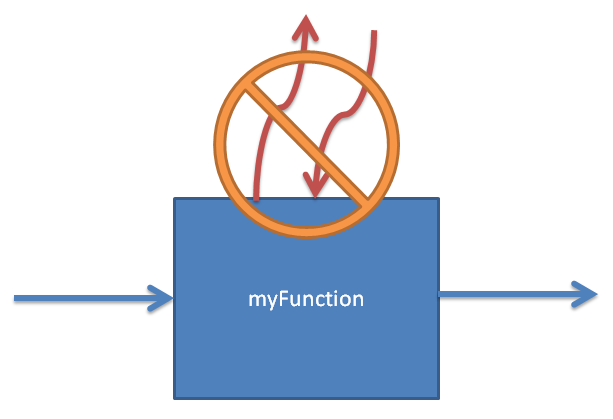
\includegraphics[width=1\linewidth]{figs/pure}
   \end{column}
   \begin{column}[]{5cm}
    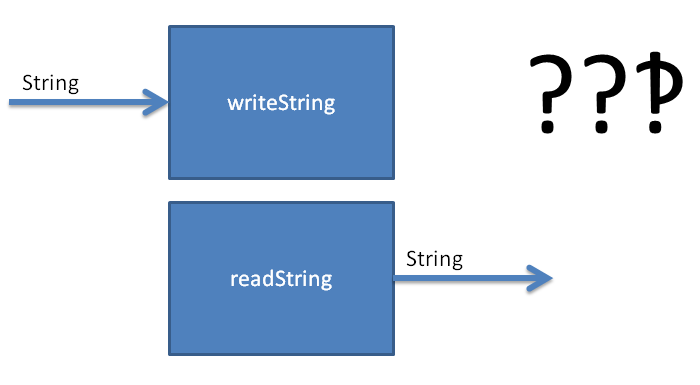
\includegraphics[width=1.1\linewidth]{figs/readWrite}
   \end{column}
  \end{columns}

\end{frame}

\begin{frame}
\frametitle{IO}
 Passing the world around 
 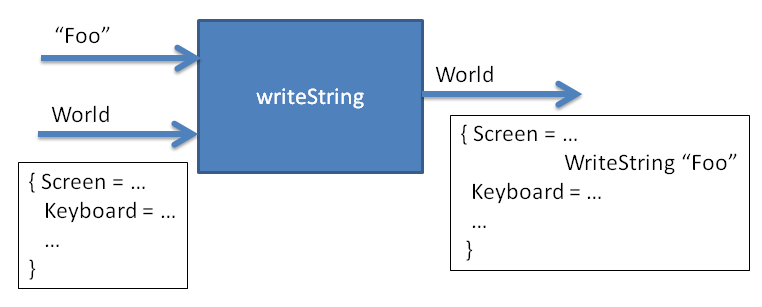
\includegraphics[width=1\linewidth]{figs/world}
\end{frame}

\begin{frame}
\frametitle{IO}
 IO operations can now be chained!
 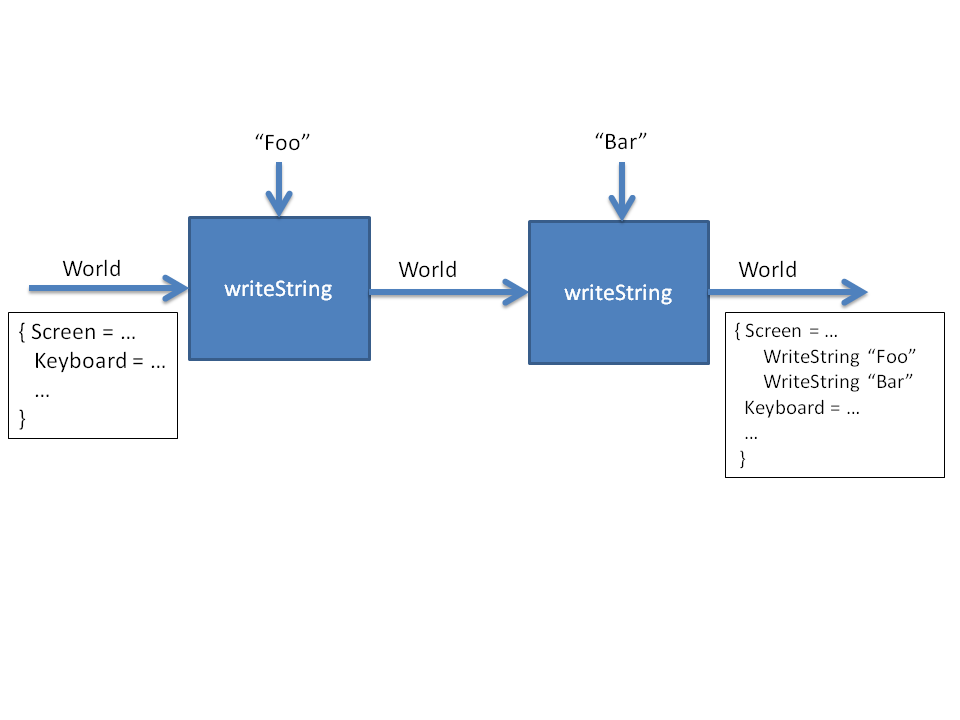
\includegraphics[width=1\linewidth]{figs/worldChain}

\end{frame}

\begin{frame}[fragile]
\frametitle{IO}
 The run-time is reading lazily the IO instructions from the output of the chain, and perform them.
 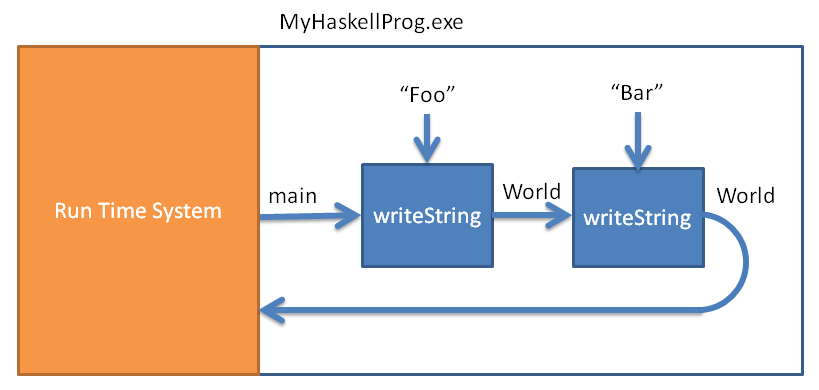
\includegraphics[width=0.8\linewidth]{figs/runTime}
 \begin{block}{Example}
  \begin{lstlisting}[basicstyle=\small]
   main = do
     putStrLn Foo
     putStrLn Bar
  \end{lstlisting}
 \end{block}

\end{frame}

\begin{frame}[fragile]
\frametitle{IO}
 readString and writeString can also interact because of lazyness.
 \vspace{0.5cm}
 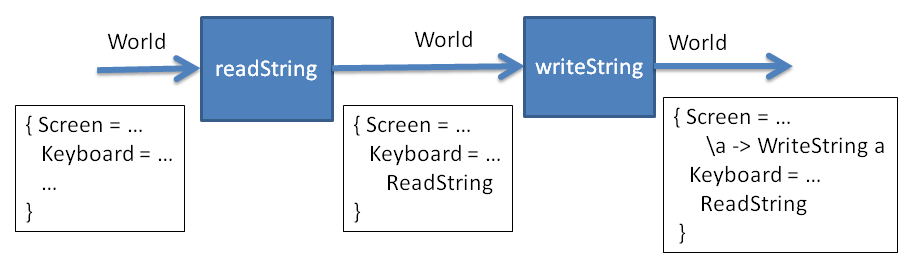
\includegraphics[width=1\linewidth]{figs/pureReadWrite}
 \vspace{0.5cm}
 \begin{block}{Example}
  \begin{lstlisting}[basicstyle=\small]
   main = do
     a <- readStrLn
     putStrLn a
  \end{lstlisting}
 \end{block}
\end{frame}


%\begin{frame}[fragile]
%\frametitle{IO}
%
% \begin{diagram}[width=300,height=200]
%  {-# LANGUAGE FlexibleContexts #-}
%  import Data.List
%  import Diagrams.TwoD.Types
%  
%  inout = arrow 1
%  box = square 1 # fc green # named "box"
% 
%  shaft  = cubicSpline False ( map p2 [(0, 0), (1, 0), (1, 0.2), (2, 0.2)])
%  
%  inIO = translate (2 ^& 1) $ rotate (90 @@ deg) $ arrow' (with & arrowShaft .~ shaft) 1
%
%  dia = inIO <> (inout ||| box ||| inout) # pad 1.3
% \end{diagram}
% 
%\end{frame}

\section{Your first program...}

%  Consolidate application/services and turn unused servers off:
%  \includegraphics[width=0.6\linewidth]{figs/VMmigration1}	\\
%  \vspace{1\baselineskip}
%  Relocate application/services to efficient servers:
%  \includegraphics[width=0.6\linewidth]{figs/VMmigration2}

\end{document}
